%#!platex jou.tex
\chapter{コマンドとマークアップ}\chaplab{cmd:and:markup}

\begin{abstract}
%{\LaTeX}はページ記述プログラミング言語です.
%ですが\Z{マークアップ}言語としての特性を活かした
%使い方を解説した説明をあまり見かけません.
%そこでまずはマークアップ言語とは何なのか,マークアップで
%何が実現できるのか,それを{\LaTeX}でどのように実現するのか
%という基本的な部分を紹介します.
マークアップ言語とは何なのか,マークアップで何が実現できるのか,
それを{\LaTeX}でどのように実現するのかという基本的な部分を紹介します.
\end{abstract}


\section{マークアップ言語とは?}
%1980年代のことでしょうか,当時文書記述言語として
%マークアップ言語というものが脚光を浴びたそうです.
今は昔,文書に対して入れ子型の論理構造を与える事によって
汎用性を持たせ,人間にも機械にも理解するのが簡単な文書の記述に関して研究
がなされたそうです\footnote{HTMLの先駆けであるSGMLが1960年代から軍事
技術の一環として研究されてきました.}.その中でもウェブページを記述する
言語してHTML: Hyper Text Markup Languageというものが出現し
たそうです.これは\Person{Tim}{Berners-Lee}らが開発し,
今はW3Cが管理しているページ記述言語です\footnote{当時は学術論文
用の記述言語という位置付けだったという話があります.}.現在は
XHTML: Extended Hyper Text Markup Languageへと進
化し,統一化が図られています.{\LaTeX}もHTMLやXHTMLと
同じようにマークアップ方式を採用しているページ記述言語です.

マークアップ型の言語にはどのような利点があるのでしょうか.
それをこの章では少し考えてみたいと思います.これを考えるには
\LaTeX の(命令・環境・宣言を含む)コマンドを観察する事から糸口が見えて
くると思いますので,コマンドに関する話を中心に進めていきます.

\begin{comment}
 これより先の話は中級編以上で扱うべきだろうと思い,まずはコマンドの基本
 的事項のみについて扱いました.
\end{comment}


\section{記号とコマンド}
{\LaTeX}はコンピュータプログラムですから,人間の意志を理解するた
めには何か特別な命令を人間から受け付けなくてはなりません.
\begin{quote}
 \yo{もしかしてこの辺は\textgt{太字}にしたいのですか?}
\end{quote}
などと対応する事はありません.皆無というわけではありませんが,
基本的にこちらから命令するまで何もしない性格です.
そのため原稿には\K{コマンド}と呼ばれる特別な\Z{記号}の綴りを使ったり,
いくつかの記号に\K{特別な意味}を持たせて使用します.ですから{\LaTeX}での
記号の意味とコマンドの役割を知っておきましょう.


\subsection{記号の分類}\zindind{記号}{の分類}%
いきなり{\laTEX}の記号の分類を考えるよりも,
普段使用している日本語や英語の記号と言語を考えましょう.
私たちはコンピュータが理解するのが難しい言語を使っています.
特に日本語はコンピュータが理解しづらいものとなっています.
それでも私たち人間は文脈などを道筋に,それらの意味を読み取ります.
\begin{quotation}
 今日は1,000円を持って,佐藤さんの商店に塩を買いに行った.
\end{quotation}
という1文を考えると,人間はすぐに\yo{1,000円}のコンマ\qu{\str,}を
\yo{お金の3桁目に入れる区切り},最後の句点\yo{.}を\yo{文の終わり}で
あると理解できます.私たちが複雑な日常文を理解できる理由として,
文の中に必ず\K{文法}が存在するという事が挙げられます.

人間はある程度
曖昧な表現を見つけてもそれを柔軟に理解できますが,コンピュータは
なにせ`1'と`0'しか分からない融通の利かない機械ですから,%\K{文法}
人間が日常的に用いている\Z{自然言語}よりは正確な文法を持った,
コンピュータが理解できる\Z{形式言語}で記述してあげる必要性があります.
%しか理解できません.正規文法については別の機会に紹介しようと
%思いますが,
%とにかく人間の使う日本語とは違いきっかりしているということです.
%この正規文法に基づいた\K{正規言語}を理解
%するのがコンピュータプログラムなわけです.{\laTEX}も正規言語
\laTEX は\Z{生成文法}を基礎とした形式言語
しか理解できませんから,ユーザから入力される記号には全て
明確な意味を持たせる必要があります.現在のバージョンの \laTEX では
曖昧な意味を持たせて文章を執筆する事はできません.

{\LaTeX}ではユーザが出力したい意味を理解するために全ての記号に
{\LaTeX}なりの意味を割り当てています.
人間がキーボードから\qu{\str<}という記号を入力しても数学の
比較演算子とは理解してくれません.\qu{\str$\str<\str$}としなければ
\yo{ここからここは数式であり,\qu{\str<}は比較演算子として使う}
という\K{意味}を理解してくれません.そのため{\LaTeX}に入力を
与えるユーザは{\LaTeX}の文法を覚える必要があります.
詳しく覚える必要はありませんが
\begin{quote}
\verb|\ { } $ & # ^ _ ~ %|
\end{quote}
という10個の記号には特別な意味がある事を覚えてください.
それぞれの記号の使い方はその時々に説明しますので,今はざっと10個
の記号が特別な意味を持ち,英文字と漢字,それに平仮名や片仮名だけが
普通の単語を作るための文字として%理解してくれると思ってください.
認識されるのだと解釈して頂いても構いません.

\begin{Trick}
\index{JIS X 0208@JIS~X~0208}%
\index{文字!半角カナ}%
\laTEX は標準的にはJIS~X~0208(JIS 第1水準・第2水準)の文字集合までしか
扱う事ができませんから,\Z{機種依存文字}や\Z{半角カナ}文字は出力できませ
ん.これらを拡張する試みがいくつかあります.近年は\Hito{齋藤}{修三郎}に
よるAdobe-Japan-1-6までの文字集合を扱える\Y{OTF}パッケージ等があります.
機種依存がどの文字かを知るために,例えばウェブで検索するのも良いでしょう.

\end{Trick}

\subsection{コマンド}\seclab{ml:command}
テキストを入力していると\qu{\str{<}}というキーボードからの入力が
\qu{!`}になってしまいます.これは一体どういう事でしょうか.考えて
みると\qu{\str{<}}という入力は\qu{\str{<}}という記号を出力するという
命令ではなく別の命令,\qu{!`}を出力するという命令に割り当てられている
と考えられます.さらに \verb|\%| のようなバックスラッシュ\pp{円}の次に
記号が来るようなコマンドも存在します.ここで{\LaTeX}のコマンドは
\yo{バックスラッシュと文字列}という形式ではない事が分かります.
正確には\yo{バックスラッシュと記号の綴り}を\K{コントロール%
シークエンス}と呼び,特殊記号1文字を\K{コントロールシンボル}
と呼びます.
{\LaTeX}におけるコマンドは大きく分けると三つに分類できます.
\begin{description}
\zindind{コントロール}{シークエンス}%
\zindind{コントロール}{シンボル}%
\zindind{コントロール}{スペース}%
\zindind{コントロール}{ワード}%
 \item[{コントロールシークエンス}]
\index{"\@\verb+\+}\glossary{"\@\verb+\+}
   バックスラッシュ\qu{\texttt\bs}\pp{\qu{\texttt\yen}}と記号の綴り.%}
   \K{制御綴り}と訳される事もあります.これを本書では%"}
   狭義の\K{コマンド}として表現しています.
 \begin{description}
   \item[{コントロールワード}] 
      バックスラッシュと英字の綴り.例えば\qu{\texttt{\bs section}}など.
   \item[{コントロールシンボル}] 
      バックスラッシュと英文字以外の綴り.例えば\qu{\texttt{\bs3}}とか
      \qu{\texttt{\bs\#}}など.
   \item[{コントロールスペース}] 
      バックスラッシュとスペース一つの綴り.\qu{\texttt{\bs}\textvisiblespace}の事.
 \end{description}
 \item[特殊記号]
   特別な意味を持つ記号.{\KY{予約文字}}と呼ばれる事も
あります.例として\qu{\texttt{\char'173}}, \qu{\texttt{\$}}など.%$
 \item[英数字など]
   バックスラッシュの付かない普通の文字列.
\end{description}
現段階では大きく分けると
\begin{itemize}
 \item バックスラッシュと文字列の綴り.
 \item 特殊な記号.\indindz{記号}{特殊な}%
 \item 普通の文字列.
\end{itemize}
の三つがある事を理解してください.本書では制御綴り
\pp{コントロールシークエンス}の事を\K{コマンド}と呼び
\K{命令},\K{宣言},\K{環境}の三つに分類します.
\begin{description}
\item[\Z{命令}] 
   特定の処理がそのときに実行されるコマンド.
   他の参考書ではこの命令の事を\K{コマンド}と呼ぶ事が
   多いようです.\K{引数}を取る事があり,その引数の事を
   \K{要素}と呼んだり,\K{オプション}と呼んだりします.
   例として \cmd{maketitle} や \cmd{section}などがあります.

\item[\Z{宣言}] 
   特定の処理がそれ以降継続して行われるコマンド.
   処理の適用される範囲を限定する\pp{\Z{グルーピング}する}事も
   できます.引数をとる事は稀.よく宣言の事も\K{命令}や
   \K{宣言方命令}とか\K{宣言型コマンド}と呼ばれます.
   例として \cmd{ttfamily}等です.宣言型のコマンドは命令に比べると
   少ないので,本書でも断り書きとして宣言型コマンドと
   呼ぶ事が多いです.

\item[\Z{環境}] 
%   \verb|\begin|\pa{何々}と\verb|\end|\pa{何々}
%   によって要素を囲むコマンド,または囲まれている領域の
%   こと.引数を取ることがあります.
%   例として\env{document}環境などがあります.
  \cmd{begin}\pa{何々} と \cmd{end}\pa{何々} に
  よって要素を囲むコマンド,または囲まれている領域の
  事.引数を取る事があります.
  例として\env{document}環境などがあります.
\end{description}


\subsection{コマンドの定義}
\zindind{マクロ}{の定義}%
\zindind{マクロ}{の再定義}%
{\LaTeX}の原稿では新しい命令などの定義をする事ができます.
\begin{Syntax}
\C{newcommand}\pa{命令}\opa{整数}\opa{標準値}\pa{定義}\\
\C{renewcommand}\pa{命令}\opa{整数}\opa{標準値}\pa{定義}
\end{Syntax}
\Cmd{newcommand}についてですが,この命令によって,
まだ定義されていない\va{命令}を新規に定義する事
ができます.

\begin{InTeX}
\newcommand{\example}{これは例です.}
\end{InTeX}

本文中で`\cmd{example}'と記述すると
%\begin{OutText}
`これは例です.'
%\end{OutText}
という出力になります.

\begin{InTeX}
\newcommand{\example}[2]{#1は#2です.}
\end{InTeX}

続いて上記の記述に基づき本文中で`\cmd{example}\verb|{ボブ}{背が高い}|'
と記述すると,
%\begin{OutText}
`ボブは背が高いです.'
%\end{OutText}
という出力になります.さらにこの \cmd{example}命令
に任意引数があっても良い事を宣言するためには次のようにしますが,
任意引数も引数の総和に勘定します.
%\begin{InOut}
%\newcommand{\example}[2][標準]{任意引数は #1
%で,必須引数は #2 です.}
%\example{それ}\\ \example[オプション]{それ}
%\end{InOut}
\begin{InOut}
\newcommand{\example}[2][未来]{%
  私は#1#2にいます.}
\example{大学}   \example{出版}\par
\example[]{大学} \example[函館]{出
版}
\end{InOut}
このように任意引数や必須引数の定義なども,
\cmd{newcommand}命令を使う事により実現できます.
定義の中で引数は\qu{\texttt\#}\va{n}として扱い,1から9までの
整数が使えます.
%このような定義が何に使えるのかと少し疑問
%に思う方がいるかも知れませんが,以下の例題をご覧ください.
%\begin{InOut}
%\newcommand{\seq}[2][n]{%
%  \{#2_{0},\ldots,\,#2_{#1}\}}
%ぶっちゃけ$\seq{a}$って$\seq[k]{x}$だよね.
%\end{InOut}
%%$
このような定義は数式の記述などに威力を発揮します.
\begin{InOut}
\newcommand{\seq}[2][n]{%
 \{#2_{0},#2_{1},\ldots,#2_{#1}\}}
数式の集合もマクロを使って$\seq{a}$や
$\seq[k]{x}$とできます.
\end{InOut}

\cmd{newcommand}では任意引数を一つしか設けるこ
とができませんが,引数は合計9個まで使う事ができます.
\Cmd{renewcommand}では一度定義した命令を再度定義する
事ができます.

さらに通常{\LaTeX}でよく見かける環境型のコマンドの
定義に関しては以下の四つの命令が使えます.
\begin{Syntax}
\C{newenvironment}\pa{環境名}\opa{引数の個数}\opa{標準値}%
 \pa{始め}\pa{終わり}\\
\C{renewenvironment}\pa{環境名}\opa{引数の個数}\opa{標準値}%
 \pa{始め}\pa{終わり}
\end{Syntax}
\Cmd{newenvironment}では環境の始めの部分と終わりの部分
を定義して,新たに環境型の命令を作成します.引数に関する
扱いは \cmd{newcommand}と同じです.
\Cmd{renewenvironment}については一度定義した環境型の
コマンドを再度定義する機能があります.

\cmd{newcommand}/\cmd{newenvironment}以外にも便利なコマンドがあります.

\begin{Syntax}
\cmd{providecommand}\pa{命令}\opa{整数}\opa{標準値}\pa{定義}\\
\Cmd{DeclareRobustCommand}\pa{命令}\opa{数値}\opa{標準}\pa{設定}
\end{Syntax}

この \Cmd{providecommand}はすでに命令が定義済みならば何もせず,もし定義
されていないならば指定された内容の通りに命令を定義する事ができます.
\cmd{DeclareRobustCommand}を使った場合は頑丈な命令を作成できます.

\begin{Prob}
次のようにアスタリスク付きで定義したコマンドと付与していない場合のコマンドの
違いを考察してください.

\begin{InTeX}
\newcommand\testargs[1]{[#1]}
\newcommand*\testArgs[1]{[#1]}
\testArgs{1行目の入力\par 2行目の入力}.
\testargs{1行目の段落\par 2行目の段落}.
\end{InTeX} 

実際にタイプセットするとエラーが表示されます.これによりアスタリスク付きで
定義した場合は複数行の段落を引数として受けとらなくなると考えられます.
\end{Prob}

\begin{Exe}
中央揃えを行い文章を強調するような \E{cemph} 環境は次のように定義します.
\begin{InOut}
\newenvironment{cemph}%
  {\begin{center}\begin{em}}%
  {\end{em}\end{center}}
ここの文章は通常通り出力され,
\begin{cemph}
この中の文章は中央揃えで強調表示
\end{cemph}
されましたか?
\end{InOut}
\end{Exe}

\begin{Prob} 
\C{DeclareRobustCommand} を使った例を示します.次のファイルをタイプセッ
 トし,その結果を吟味してください.

\begin{InTeX}
\documentclass{jarticle}
\DeclareRobustCommand{\joubuyen}{{\ooalign{Y\crcr\hss=\hss}}}
\newcommand{\moroiyen}{{\ooalign{Y\crcr\hss=\hss}}}
\begin{document}
\tableofcontents
\section{もろい{\moroiyen}は壊れやすい}
どうですかねぇ。
\section{丈夫な{\joubuyen}は壊れにくい}
大丈夫ですか?
\end{document}
\end{InTeX}

この例では1回目のタイプセットでエラーが表示されます.

\begin{OutTerm}
! Illegal parameter number in definition of \reserved@a.
<to be read again> \crcr
l.6 \section{もろい{\moroiyen}は壊れやすい}
?
\end{OutTerm}

さらに2回目のタイプセットでは目次
ファイル\Va{file}{toc}が作成され,それが読み込まれるので
さらにエラーとなります.\Va{file}{toc}と\Va{file}{aux}に
何が記述されているのかを吟味してください.\Va{file}{aux}には
次のように出力されており,凄い事になっています.

\begin{InTeX}
\relax
\@writefile{toc}{\contentsline{section}{\numberline{1}もろい
  {{\lineskiplimit -\maxdimen \unhbox \voidb@x \vtop {\baselineskip 
  \z@skip \lineskip .25ex\everycr{}\tabskip \z@skip \halign {##\crcr
  Y\crcr \hss =\hss \crcr }}}}は壊れやすい}{1}}
\@writefile{toc}{\contentsline{section}{\numberline{2}丈夫な
  {\joubuyen}は壊れにくい}{1}} 
\end{InTeX}

さらに\Va{file}{toc}には次のような出力になります.

\begin{InTeX}
\contentsline{section}{\numberline{1}もろい{{\lineskiplimit 
  -\maxdimen \unhbox\voidb@x \vtop {\baselineskip \z@skip 
  \lineskip .25ex\everycr{}\tabskip \z@skip \halign {####\crcr 
  Y\crcr \hss =\hss \crcr}}}}は壊れやすい}{1}
\contentsline{section}{\numberline{2}丈夫な{\joubuyen}
  は壊れにくい}{1}
\end{InTeX}

これが \cmd{DeclareRobustCommand}で \cmd{moroiyen}命令
を定義しなかった結果となります.{\LaTeX}の命令を
何か別のファイルに書き出す場合は丈夫な命令として定義して
いた方が無難なようです.ただし,次のように \Cmd{protect}
命令を使った場合はうまく行く事を確認してください.

\begin{InTeX}
\section{もろい{\protect\moroiyen}は壊れやすい} 
\end{InTeX}

\Cmd{protect}を使うと \cmd{moroiyen}が壊れずに
\Va{file}{toc}や\Va{file}{aux}に出力されている事も
確認してください.
\end{Prob}

%このような定義をするコマンドのほかに{\LaTeX}では
%数値を操作するコマンド,組版に関するコマンドなど
%数多く存在します.
%
%以上のことを踏まえてこれからマクロとクラスについての
%解説をします.各章並びに各節は用途別にそれらを分類し,
%必要に応じて相互参照をしています.また,索引からもパ
%ッケージやクラス,コマンドなどを追うことができます.


\subsection{文字やコマンドの区切り}\seclab{moji:kugiri}

私たち人間はある文や節の区切りをどのように判断しているのでしょうか.一つ
は文と文のあいだや単語と単語のあいだに挿入される空白です.空白は文字列の
区切りを示し,その空白には意味の区切りがあります.では節はどうで
しょうか.例えば日本語では
\begin{quote} 
 \yo{公園の中のベンチのうえ}
\end{quote}
という名詞があったとすると,これはそれぞれ
\begin{quote}  
 \yo{公園}\yo{の}\yo{中}\yo{の}\yo{ベンチ}\yo{の}\yo{うえ}
\end{quote}
に分けて文を解釈し,{\KY{名詞}}や{\KY{助動詞}}など
の{\KY{品詞}}に分ける事ができます.

もう一つの例としてメールアドレスの場合を考えて見ましょう.
メールアドレスはそもそもコンピュータ上で手紙のやり取りを
するための住所ですからコンピュータが分かりやすい
表現になっていますが,人間にも分かりやすい表記になっています.
仮に
\begin{quote}
\verb|name@server.co.jp|
\end{quote}
というメールアドレスがあったとします.するとこれは
\begin{quote}
\qu{\str{name}} \qu{\str{@}} \qu{\str{server}}
\qu{\str{.}} \qu{\str{co}} \qu{\str{.}} \qu{\str{jp}}
\end{quote}
に分けられます.それぞれ
\begin{description}
 \item[\str{name}] メールアドレスを使っている人の\yo{名前}.
 \item[\str{@}]   \qu{\str@}は\qu{at}の意味でもあって,これ以降の文字は\yo{住所}を
	    表す事を示す.
 \item[\str{jp}] その人の\yo{国}を表す.
 \item[\str{co}] その人がどんな\yo{地域\pp{組織}}に所属しているのかを表す.
 \item[\str{server}] 地域の中のどこにいるのかをあらわす住所.
 \item[\str{.}] 住所を区切るために使われている.
\end{description}
という意味合いを持っています.住所の区切りが空白ではなくピリオドなのは
仕方のない事です.コンピュータの世界ではなるべく文字列は
空白を含んでいないほうが処理が行いやすいのです.
さて,これはどのようにして区切りを見つけたのでしょうか.
メールアドレスの例では\qu{\str{@}}や\qu{\str{.}}を文字の区切りとして
住所を判定しています.{\LaTeX}でも同じような事をやっています.

では文字列としてのコマンドが{\LaTeX}でどのように解釈されるのかを
考えてみましょう.ここでは引数を取る命令を考えてみます.
まずは次のような入力の出力を予想してみましょう.

\begin{InTeX}
\newcommand{\OneArg}[1]{あ,#1だよ}
\OneArg ほあれそれ.
\end{InTeX}

結果は\yo{あ,ほだよあれそれ.}です.
この結果から{\LaTeX}では引数には何も指定がなければ1文字しか受け取らない
という事が分かります.
%という定義がマクロの中では可能なので,ユーザから \cmd{hoge}命令の
%実態を隠すことができます.
%これは開発者と使用者の分離を行うために
%仕方がないのですが,逆に使用者が自分の思い通りに
%命令をカスタマイズできないとか,様々な不満があるようです.

続いて次のようにしてみましょう.

\begin{InTeX}
\newcommand{\OneArg}[1]{あ,#1だよ}
\OneArg {あれそれ},それ.
\end{InTeX}

結果は\yo{あ,あれそれだよ,それ.}になるでしょう.
どうやら引数を波括弧\qu{\texttt{\lb\space\rb}}で囲むと
\K{それを一つの文字の塊として}受け取るようです.

次に二つ引数を取る命令を定義します.

\begin{InTeX}
\newcommand{\twoArgs}[2]{あ,#1だよ,ほら#2}
\twoArgs       {それ}          ね.
\end{InTeX}

この場合の結果は\yo{あ,それだよ,ほらね.}となるでしょう.
もうお分かりですね.{\LaTeX}の引数に複数の文字列を渡したいときは
括弧でグルーピングすれば良いのです.

さて今度は(\TeX の世界では通常の)文字ではない\qu{\str{@}}を含む命令を
定義してみましょう.

\begin{InTeX}
\newcommand{\two@args}[2]{あ,#1だよ,ほら#2}
\two@args       {それ}          ね.
\end{InTeX}

これをタイプセットするとエラーになるので
\keytop{Enter}キーを4回ほど押すとエラーが表示されるでしょう.

\begin{OutTerm}
! Missing number, treated as zero.
<to be read again>
                   g
l.7 \newcommand{\two@args}[2]{あ,#1だよ,ほら#2}
?
! You already have nine parameters.
\reserved@a ...def \expandafter \h \reserved@b #10
                                                  g{
l.7 \newcommand{\two@args}[2]{あ,#1だよ,ほら#2}
?
! You can't use `macro parameter character #' in horizontal mode.
<argument> あ,##
                 1だよ,ほら##2
l.7 \newcommand{\two@args}[2]{あ,#1だよ,ほら#2}
?
! You can't use `macro parameter character #' in horizontal mode.
<argument> あ,##1だよ,ほら##
                              2
l.7 \newcommand{\two@args}[2]{あ,#1だよ,ほら#2}
?
\end{OutTerm}


これは一体どういう事でしょうか.%
\indindz{区切り}{コマンドの}%%
メールアドレスの例を思い出してほしいのですが,{\LaTeX}ではどうや
ら\qu{\str{@}}をコマンドの区切りとして解釈しているようです.

\begin{InTeX}
\newcommand{\h}[2]{あ,#1だよ,ほら#2}
\two@args       {それ}          ね.
\end{InTeX}

そして引数の受け取り方を考えた場合の結果は\yo{あ,@だよ,ほらgeそれね.}
となる事でしょう.

この事から{\LaTeX}においての命令の定義には英字のみに
する事が求められるようです.そして英字以外の文字列は,
そこをコマンドの区切りとして英字以外の文字列を引数として
受け取るという事です.

この文字の分類を利用して{\LaTeX}ではマクロの中において特別な
処理をしています.マクロは容易に変更してもらっては困るので
ユーザからそのマクロを簡単に変更されないようにしています.
その方法の一つとしてマクロの中では\Z{アットマーク}\qu{\str{@}}を英字と同じ分類\index{"@@\verb+"@+}%
として扱うのです.\qu{\str{@}}を英字と同じ分類にすると,
そこでコマンドは区切られないので次のように \cmd{two@args} が定義できる
わけです.

\begin{InTeX}
\newcommand{\two@args}[2]{あ,#1だよ,ほら#2}
\end{InTeX}

そして \cmd{two@args} の定義がマクロの中では可能なので,
ユーザから \cmd{twoArgs} 命令の実態を隠す事ができます.

\begin{InTeX}
\newcommand{\two@args}[2]{あ,#1だよ,ほら#2}
\newcommand{\twoArgs}{\two@args}
\end{InTeX}

これは開発者と使用者の分離を行うために
仕方がないのですが,逆に使用者が自分の思い通りに
命令をカスタマイズできない等,様々な不満があるようです.

実際ヘッダーやフッターを自分流にカスタマイズしたいときは
それらの命令に\qu{\str{@}}が含まれているために変更できない,
という事態に陥ります.マクロで行っている事,\qu{\str{@}}を
英字と同じ分類にしてコマンドを定義するためには
\begin{Syntax}
\Cmd{makeatletter} \pp{\qu{\str{@}}を英字と同じ分類にする.}\\
\Cmd{makeatother}  \pp{\qu{\str{@}}を違う分類にする.}
\end{Syntax}

`\str{@}'を含むコマンドに関しては上記の二つの命令を使います.
この命令の中身を見てみると実は次のようになっています.

\begin{InTeX}
\def\makeatletter{\catcode`\@11\relax}
\def\makeatother{\catcode`\@12\relax}
\end{InTeX}

\indindz{コード}{カテゴリー}\indindz{コード}{分類}%%
どうやら\qu{\str{@}}の{\KY{カテゴリーコード}}
というものを11にすると英字と同じになり,12にすると違う分類に
なるようです.このような記号の分類を{\KY{カテゴリーコード}}と
呼びます\pp{\tabref{catcode1}参照}.

\begin{table}[htbp]
\begin{scenter}
\index{改行@行末文字としての\zdash}%}"
\index{" @\verb*+ +}
\index{"#@\verb+#+} 
\index{"$@\verb+$+}\glossary{"$@\verb+$+}
\index{"&@\verb+&+}\glossary{"&@\verb+&+}
\index{"\@\verb+\+}\glossary{"\@\verb+\+}
\index{"^@\verb+^+}\glossary{"^@\verb+^+}
\index{"_@\verb+_+}\glossary{"_@\verb+_+}
\index{"{1"}@\protect\bgroup\verb+"{+"}}
\glossary{"{1"}@\protect\bgroup\verb+"{+"}}
\index{"{2"}@"{\verb+"}+\protect\egroup}
\glossary{"{2"}@"{\verb+"}+\protect\egroup}
\index{"~@\verb+~+}
\glossary{"~@\verb+~+}
\index{%@\verb+%+}
\glossary{%@\verb+%+}
% {, }, @ | ! " 
\caption{カテゴリーコードの一覧}\tablab{catcode1}
\begin{tabular}{*3l} 
\TR
\Th{カテゴリ} & \Th{意味}        & \Th{標準での割り当て}   \\ 
\MR
%0  & エスケープ文字    & \verb|\| \pp{\ttfamily\yen}\\
%1  & グループの開始    & \verb|{| \\
%2  & グループの終わり  & \verb|}| \\
%3  & 数式モードの制御  & \verb|$|  \\
%4  & 配列の要素の区切り& \verb|&|\\%&
%5  & 行末文字          & \va{改行} \pp{\HEXCODE{0D}} \\
%6  & パラメータ文字    & \verb|#|  \\
%7  & 上付き文字        & \verb|^|  \\
%8  & 下付き文字        & \verb|_|  \\
%9  & 無視される文字    & なし${}^{*1}$\\
%10 & 空白              & \verb*| | \\
%11 & 英文字            & \str A$\cdots$\str Zと\str a$\cdots$\str z\\
%12 & そのほかの文字    & \verb| ( ! ? 1 2 @|など\\
%13 & アクティブ文字    & \verb|~| \\
%14 & コメント文字      & \verb|%| \\
%15 & 無効文字          & \va{デリート} \pp{\HEXCODE{7E}}\\
0  & \Z{エスケープ文字}    & \verb|\| \pp{\ttfamily\yen}\\
1  & グループの開始    & \verb|{| \zindind{グループ}{の開始}\\
2  & グループの終わり  & \verb|}| \zindind{グループ}{の終わり}\\
3  & 数式モードの制御  & \verb|$|  \\
4  & 配列の要素の区切り& \verb|&| \zindind{配列}{の要素の区切り} \\%&
5  & {行末文字}          & \va{改行} \pp{\str{0x0D}} \zindind{行末}{文字}\\
6  & {パラメータ文字}    & \verb|#|  \zindind{パラメータ}{文字}\\
7  & \Z{上付き文字}        & \verb|^|  \\
8  & {下付き文字}        & \verb|_|  \zindind{下付き}{文字} \\
9  & \Z{無視される文字}    & なし${}^{*1}$\\
10 & \Z{空白}              & \verb*| | \\
11 & \Z{英文字}            & \str A$\cdots$\str Zと\str a$\cdots$\str z\\
12 & そのほかの文字    & \verb| ( ! ? 1 2 @|など\\
13 & \Z{アクティブ文字}    & \verb|~| \\
14 & {コメント文字}      & \verb|%| \zindind{コメント}{文字}\\
15 & \Z{無効文字}          & \va{デリート} \pp{\str{0x7E}}\\
\MR
\multicolumn{3}{c}{\Th{以下三つは日本語{\TeX}のもの}}\\
\MR
16 & 第1・第2水準の漢字      & 亜,丼など\\
17 & かな,全角アルファベット& あ,ア,a,Aなど\\
18 & その他の全角記号        & ┼,【など\\
\BR
\end{tabular}
\\ {\small ${}^{*1}$標準では割り当てられていない}%$
\end{scenter} 
\end{table}

そのため何かマクロの中のコマンドに自分で変更を加えたいときは
\qu{\str{@}}を含む箇所を \cmd{makeatletter}
と \cmd{makeatother}で囲んであげます.

\begin{InTeX}
\documentclass{jsarticle} 
\makeatletter
\newcommand{\two@args}[2]{あ,#1だよ,ほら#2}
\newcommand{\twoArgs}{\two@args}
\makeatother
\begin{document}
\twoArgs{それ}{ね}.
\end{document}
\end{InTeX}


\begin{Exe}
\C{@ifstar}は `\str @'を含む命令で,引数の始めにアスタリスク(星)`\str{*}'が
あるかどうかを判定します.次の例の実行結果を吟味してください.

\begin{InTeX}
\newcommand\checkstar{\@ifstar{星付き}{星なし}}
\checkstar, \checkstar*, \checkstar!.
\end{InTeX}

上記の例を実行すると次のようなエラーが表示されます.

\begin{OutTerm}
! You can't use `\spacefactor' in vertical mode.
\end{OutTerm}
\index{You can't use `spacefactor'@\texttt{You can't use
 `\bs spacefactor' in vertical mode}}%
\index{エラー!You can't use ``spacefactor'@\texttt{You can't use
 `\bs spacefactor' in vertical mode}}


やはり`\str @'を含む命令を用いるには \C{makeatletter} と \C{makeatother}
で囲む必要があるようです.以下のように修正し,その実行結果を吟味
してください.

\begin{InTeX}
\makeatletter
\newcommand\checkstar{\@ifstar{星付き}{星なし}}
\checkstar, \checkstar*, \checkstar!.
\makeatother
\end{InTeX}
% 星は \C{@ifstar} に持っていかれます.
\end{Exe}

\subsection{コマンドの引数}
%引数と取るコマンドに対して文字列を渡した場合の
%挙動は予想しやすいと思います.ではコマンドに対して
%コマンドを渡した場合はどうなるでしょうか.
%\begin{InOut}
%\newcommand{\twoarg}[2]{一つ目の#1,二つ目の#2}
%\twoarg a bとか\twoarg{それ}{げほ}とか,
%さらに\twoarg{\LaTeX}{\LaTeXe}は?
%\end{InOut}
%どうやら引数を取るコマンドに対してさらにコマンドを
%引数に与えても良いようです.では次の場合はどうでしょうか.
%\begin{InOut}
%\newcommand{\twoarg}[2]{一つ目の#1,二つ目の#2}
%ほほう\twoarg\LaTeX\LaTeXe とは粋だね.
%では\twoarg\LaTeX2\LaTeXe はどうだね?
%\end{InOut}
引数を取るコマンドに対して文字列を渡した場合の
挙動は予想しやすいと思います.ではコマンドに対して
コマンドを渡した場合はどうなるでしょうか.
\begin{InOut}
\newcommand{\twoarg}[2]{#1! #2? }
\twoarg a bとか\twoarg{はこだて}
{未来}とか,さらに\twoarg{\LaTeX}
{\LaTeXe}
\end{InOut}
どうやら引数を取るコマンドに対してさらにコマンドを
引数に与えても良いようです.では次の場合はどうでしょうか.
\begin{InOut}
\newcommand{\twoarg}[2]{#1! #2? }
\twoarg\LaTeX\LaTeXe 
\twoarg\LaTeX2\LaTeX3
\end{InOut}
これは\secref{moji:kugiri}で行った内容が含
まれています.\qu{\LaTeX}と\qu{2}のあいだで語が区
切られて解釈されているので二つ目の引数に\qu{2}
だけが渡されています.

%\subsection{コマンド定義中の空白の扱い}
%コマンドを定義するための命令 \cmd{newcommand}の中では
%空白が無視されるわけではありません.次の出力の違いを
%見比べてください.
%\begin{InOut}
%\newcommand\kuhaku[1]{それと   #1だ,}
%\newcommand\Kuhaku[1]{それと#1だ.}
%\kuhaku{だめ} \Kuhaku{だめ   }
%\end{InOut}
%この例では空白が二つ以上続いており,それらが一つの空白として
%解釈されて,引数と文のあいだに余分な空白が挿入されています.
%正しくは
%\begin{InOut}
%\newcommand\kuhaku[1]{それと#1だ,}
%\newcommand\Kuhaku[1]{それと#1だ.}
%\kuhaku{だめ} \Kuhaku{だめ}
%\end{InOut}
%のように定義したほうが良いようです.

%ただ例外もあって空白を吸収するコマンドの後に
%空白があっても余分が空白は挿入されません.
%\begin{InOut}
%\newcommand{\chisai}[2]{{\small#1}{\Large#2}}
%あれ,\chisai{  それ}{げほ}は\chisai{  だめ}{ろう}.
%\end{InOut}
%上記の例では\Cmd{relax}という命令が使われていま
%すが,これを取り除くとどうなるでしょうか.

\section{グルーピング・入れ子構造}
\indindz{スコープ}{変数の}
{\laTEX}は\Z{変数}の\Z{スコープ}\pp{有効範囲}というプログラミングでは
当たり前の機能を持っています.これはプログラミングをやった事のない人
には馴染みの薄いものなので詳しく説明しましょう.

まず変数には\yo{限られた範囲だけ有効}
な{\KY{局所変数}}と\yo{全ての範囲で}
有効な{\KY{大域変数}}の2通りがあります.
{\LaTeX}においてもこれは重要な話で
,この有効範囲\pp{\K{スコープ}}を決めるのが
\Z{波括弧}です.

方言のように地方によってアクセントや
言葉が違う事がありますが,{\LaTeX}
でも地方\pp{範囲}を分けて言葉\pp{定義}の
使い分けができます.以下の例題をご自分
で試してみてください.

\begin{InTeX}
\newcount\test%          新規に変数の調達
\the\test%               変数の値を表示
{%                       グループ1の開始
   \test=3 \the\test%    \testに3を代入して値を表示
   {%                    グループ2の開始
      \test=5 \the\test% \testに5を代入して値を表示
   }%                    グループ2の終了
   \the\test%            グループ2で testに5を代入しても?
}%                       グループの終了
\the\test%               ここでの値は?
\test=6 \the\test%       \testの値は?
\end{InTeX}

\cmd{newcount}は新規にカウンタ\pp{レジスタ}を用意し,
\Cmd{the}はカウンタなどの値を表示する命令です.
さて,以上の入力から\yo{035306}と
いう値を得る事ができたでしょうか.
この事を考えると\yo{内側の括弧で代入した値は外側の
括弧の領域に影響しない.}という事であり,\yo{外側で値を
変更しても内側の括弧にある値まで変更できない}という
事です.まさに\yo{グループ}を作ってその中で好き勝手にやって
いるわけです.

次に書体変更の宣言でどのように書体が変更されるのかを
見てみましょう.今回はファミリーを変える \cmd{ttfamily}と
シェープを変える \cmd{itshape},そして普通の書体に戻
す \cmd{normalfont}という三つの宣言を使います.
\begin{InOut}
roman {\ttfamily tt {\itshape it}
 tt \normalfont it} roman
\end{InOut}
ここでおやっと気づいていただきたいのは \cmd{ttfamily}という宣言が二つの
括弧の中にまで影響しているという点です.先ほどの変数の代入ではこのように
はなりませんでした.どうやら書体の宣言は,その宣言をした場所から内側の括
弧までもが有効範囲になっているようです.これは現在の{\LaTeX}の仕様です.
宣言ではなく命令としても結果は同じになります.

\begin{InOut}
roman \texttt{ tt \textit{it}
 tt \normalfont it} roman
\end{InOut}
しかし \cmd{normalfont}命令を使うとタイプライタ体の有効範囲でも
そこで通常の書体に戻ってしまいます.こう考えると影響を
与えたくない括弧の内側の領域には \cmd{normalfont}を
使うと良い事になります.
\begin{InOut}
roman {\ttfamily tt {\normalfont
  \itshape it} tt} roman\par
roman \texttt{tt {\normalfont
  \textit{it}} tt} roman
\end{InOut}

命令ではなく宣言型のコマンドのいくつかは括弧の内側まで
影響するので,その属性を受けないようにするための工夫が
必要になります.

\subsection{大域化}
書体の属性を変更する宣言型のコマンドはスイッチの
変更をしている特殊なものでした.ここでは最初の
大域変数と局所変数の二つをもう一度見直しておきましょう.

括弧の内側で定義した内容を外側でも有効にしたいときは
どうすれば良いでしょう.また括弧の外側の定義を内側にも
有効にする方法がないと不便でしょう.\yo{用紙サイズ}
のようにそう簡単に変わってほしくない変数は括弧の内側
でも有効であってほしいものです.それらを括弧の内側で
も有効にする事を{\KY{大域化}}\pp{{\KY{グローバル化}}}
と言います.{\laTEX}においても大域化のための \cmd{global}
という命令が用意されています.

\begin{InTeX}
\newcount\test \the\test
{%グループ1
   \global\test=3  \the\test% 大域に代入
   {%グループ2
      \the\test
      \test=5 \the\test
   }
   \the\test
}
\the\test
\test=6 \the\test
\end{InTeX}

とした場合は\qu{0 3 35 3 36}となるでしょうか.3行目で大域的に
\qu{3}を代入していますので内側の括弧にも有効ですし,グループ2を
出た後の数値も\qu3です.そしてグループ1を抜けた後でも\qu3が
代入されています.以上のように \cmd{global} を使うとその
グループの内側と外側の全ての処理に影響します(\LaTeX
において,いくつかの数値を操作する命令は、あらかじめ大域化
するように定義されています).

\section{宣言と命令の違い}
例えば\env{center}環境のコマンドを考えると,
なぜ環境の内側では全ての行が中央揃えになるのでしょう.
一つは始めと終わりをグループにする事で,どこからどこまでが中央揃えなのか
が分かっているのでしょう.

`\verb|\begin{center}|'によってグループが始まり,
`\verb|\end{center}|'によってグループの終わりが示されています.

\yo{\K{これをまさに中央揃えにしてください.}}
と言うよりは\yo{\K{ここからここまでを中央揃えにしてください}}
というコマンドのほうが都合が良い事に気づくでしょう.
\C{centering}命令を使うと次のようになります.

\begin{InTeX}
{\centering A long long ago, a man was doing any test...} 
\end{InTeX}

しかし,非常に長い文章の場合は \cmd{centering} 命令を使うよりは,
\env{center}環境としてグループ化したほうが分かりやすいでしょう.

\begin{InTeX}
\begin{center}
 A long long ago, a man was doing any test...
\end{center}
\end{InTeX}

そう考えるとコマンドには次の二つがある事が分かります.

\begin{description}
\indindz{コマンド}{宣言型の}%
\indindz{コマンド}{命令型の}%
\zindind{宣言}{型のコマンド}%
\zindind{命令}{型のコマンド}%
 \item[{宣言型コマンド}] 使用してからそれ以降ずっと有効
	    なコマンド.環境型のコマンドに使われたり,
	    単独で使われる.
 \item[{命令型コマンド}] 使用した場所で有効なコマンド.
	    通常は引数に与えられたものを処理する.
\end{description}


例として命令型の \cmd{textsf} と宣言型の \cmd{sffamily} を
考えてみましょう.命令型の場合は次のような使い方はできません.

\begin{InTeX}
Roman. \textsf{Roman? \par This is sans serif family.} Roman!
\end{InTeX}

ただし,宣言型ならば新規に\env{sffont}環境を定義できます.

\begin{InOut}
\newenvironment{sffont}{\sffamily}{}
Roman.
\begin{sffont} 
   Roman? \par This is sans serif.
\end{sffont}
\par Roman!
\end{InOut}

宣言型のコマンドはそれ以降ずっと有効なので有効範囲を
決めてあげます.\cmd{sffamily}などの書体を変更する
コマンドはグルーピングする必要があります.
\begin{InOut}
Roman! {\sffamily sans serif.}
Roman!
\end{InOut}

\begin{Trick}
今まで使ってきた \cmd{begin}\pa{何々} と \cmd{end}\pa{何々} 
というコマンドは,このグルーピングの作業をやってくれているの
です.補足的な事ですが
%\begin{InTeX}
%\begin{<何々>}  <要素> \end{<何々>}
%\end{InTeX}
\begin{Syntax}
\cmd{begin}\pa{環境名} \va{要素} \cmd{end}\pa{環境名}
\end{Syntax}
というのは{\LaTeX}側で
%\begin{InTeX}
%{\何々 <始めの処理>  <要素> <終わりの処理>}
%\end{InTeX}
%\begin{Syntax}
`\texttt{\lb \va{コマンド} \va{始めの処理} \va{要素} \va{終わりの処理}\rb}'
%\end{Syntax}
に解釈されるので \cmd{sffamily} のような宣言も
\begin{InOut}
Roman?
\begin{sffamily} 
This is sans serif family.\par
\end{sffamily} 
Roman!
\end{InOut}
とできます.こうすると特に長い文章が読みやすくなります.
\end{Trick} 

\section{相互参照}\seclab{xr}
文章の論理構造を明確にしてくれるものの一つに{\KY{相互参照}}
があります.相互参照の仕方は参照したいものに\Z{ラベル}を貼り,
挿入したい場所でラベルを参照するという二つの作業に分けられま
す.相互参照できる項目は以下の四つ程に限られています.
\zindind{相互参照}{できるもの}%
\begin{itemize}
\item  章節命令 \pp{{\texttt{\bs section}}命令など}
\item  番号付き数式 \pp{\env{equation}環境など}
\item  \texttt{float}環境の要素\pp{図や表など}
\item  \texttt{enumerate}環境内の個々の項目
\end{itemize}
要は通し番号のついているものには付けても良いようです.
ラベルは単純に貼りたいものに \Cmd{label} 命令で次のように使用します.
\begin{Syntax}
\va{参照したい要素}\Cmd{label}\pa{ラベル名}
\end{Syntax}

参照の仕方にはその番号を参照する \Cmd{ref} とページを参照す
る \Cmd{pageref}の2通りがあります.
\begin{Syntax}
\begin{tabular}{ll}
 \cmd{ref}\pa{ラベル}     &\pp{通し番号}\\
 \cmd{pageref}\pa{ラベル} &\pp{ページ番号}\\
\end{tabular}
\end{Syntax}
参照の仕方は以下のようになります.通し番号を参照す
る \cmd{ref} 命令は \cmd{section} 命令のようなものを参照するとき
に非常に便利です(\cmd{section}の行頭のコメントは外してください).
\begin{InOut}
%\section{相互参照}\label{sec:xr}
詳しくは\pageref{sec:xr}~ページの
\ref{sec:xr}~節で述べているのでそ
ちらを参照されたい.
\end{InOut}

\zindind{目次}{の作成}
相互参照や目次を作成しているときはタイプセットを3回程行
う必要があります.ラベルの名前が重複しないように工夫する
事も必要です.


% test test test
\subsection{相互参照の仕組み}\zindind{相互参照}{の仕組み}%
節\pp{見出し}や図表には通し番号を付けます.これは同じ名前の節 
\pp{見出し}が同じページに存在しても区別できるという利点があり
ます.そして節\pp{見出し}を参照するときはその番号を示します.
このような機能を実現するために{\LaTeX}では{\KY{カウンタ}}を使いま
す.ユーザが特にこの事を意識しなくても半自動的に番号付
けなどをやってくれます.一応さわり程度にはその仕組みを説明
します.

相互参照する対象が通し番号ですので,節なら節などの要素に応
じたカウンタがあらかじめ用意されています.{\LaTeX}では
\tabref{latexcounters}の通りにあらかじめ定義されている
カウンタがあります.
\begin{table}[htbp]
\begin{scenter}
\indindz{番号}{見出しの通し}\indindz{番号}{図表見出しの通し}%%
\caption{あらかじめ定義されているカウンタ名}\tablab{latexcounters}
\begin{tabular}{*3l}
 \TR
  \Th{カウンタ名}      & \Th{割り当て} \\
 \MR
 \Kount{part}          & 部見出し \\
 \Kount{chapter}       & 章見出し \\
 \Kount{section}       & 節見出し \\
 \Kount{subsection}    & 小節見出し\\
 \Kount{subsubsection} & 小小節見出し\\
 \Kount{paragraph}     & 段落見出し\\
 \Kount{subparagraph}  & 小段落見出し\\
 \Kount{page}          & ページ番号\\
 \Kount{equation}      & 式番号\\
 \Kount{figure}        & 図見出し\\
 \Kount{table}         & 表見出し\\
 \Kount{footnote}      & 脚注番号\\
 \Kount{mpfootnote}    & \env{minipage}環境中の脚注番号\\
 \Kount{enumi}         & 一つ目の階層の\env{enumerate}環境の番号\\
 \Kount{enumii}        & 二つ目の階層の\env{enumerate}環境の番号\\
 \Kount{enumiii}       & 三つ目の階層の\env{enumerate}環境の番号\\
 \Kount{enumiv}        & 四つ目の階層の\env{enumerate}環境の番号\\
 \BR
\end{tabular}
\end{scenter}
\end{table}
カウンタは\yo{素の番号}と実際に出力すべき\yo{表示用の番号}
と\yo{参照用の文字列}の三つの要素を持っています.
例えば `\verb|\newcounter{section}[chapter]|'
というのは,おおよそ次のような処理と同じ事になります(\C{newcounter}と
は新しいカウンタを定義するための命令です.).

\begin{InTeX}
\newcount\c@section %素の番号用
\def\thesection{\thechapter.\c@section}%表示用
\def\p@section{\thechapter.\c@section}%参照用
\end{InTeX}


%\begin{description}
% \item[\cmd{c@table}] 
%	    素の番号を保存する\kount{table}用カウンタ.
% \item[\cmd{thetable}] 
%	    章の子カウンタである表示用の命令.
% \item[\cmd{p@table}] 
%	    参照用の命令.
%\end{description}
%の三つが同時に定義されることになります.

%\begin{InTeX}
%\label{test}, \ref{test} 
%\end{InTeX}

この仕組みについて理解するには実際の動作を見るのが早いと思います.
ファイル名\fl{reftest.tex}というファイルを作成し,1回だけタイプセットして
ください.

\begin{InTeX}
\documentclass{jsarticle}
\begin{document}
\newcounter{test} \thetest
\refstepcounter{test} \thetest
\end{document}
\end{InTeX}


ここで \cmd{refstepcounter}はカウンタの値を一つ増やす命令
で \cmd{thetest}はカウンタ\kount{test}の値を表示するための
命令だと思ってください.
結果として端末には \dos{No file reftest.aux} というメッセージが表示され
るはずです.この段階で\fl{reftest.aux}を\prog{cat}か\prog{type}
コマンドで見ると次の1行しか出力されていません.

\begin{InTeX}
\relax 
\end{InTeX}

\cmd{refstepcounter}命令だけでは参照できる状態にはないようです.

\begin{InTeX}
\refstepcounter{test} \thetest
\end{InTeX}

上記の1行に対して次のように`\verb|\label{cnt:test}|'を書き足して,
1回だけタイプセットを行ってください.

\begin{InTeX}
\refstepcounter{test} \thetest \label{cnt:test}
\end{InTeX}


\begin{flushleft}
\dosh{Label(s) may have changed. Return to get cross-ferecenses right.} 
\end{flushleft}
端末にはこのような{\LaTeX}の警告が表示されます.ラベルが変更されたと
思われるので解消しなさいと言われています.ここで
\fl{reftest.aux}を見ると \C{newlabel}命令という新しい情報が出力されています.

\begin{InTeX}
\relax
\newlabel{cnt:test}{{1}{1}}
\end{InTeX}


これで\str{cnt:test}という名前のラベルを参照する準備が
できている事が分かります.

\begin{InTeX}
\newcounter{test} \thetest
\refstepcounter{test} \thetest \label{cnt:test}
\end{InTeX}

上記の2行に対して \cmd{ref} と \cmd{pagref}を含むような,次の1行を付け足
して1回だけタイプセットします.

\begin{InTeX}
ref=\ref{cnt:test}, page=\pageref{cnt:test}
\end{InTeX}

するとコンソールに警告は表示されません.\fl{reftest.aux}の内容も変わって
いません.さて,ここで{\LaTeX}に意地悪をするため,
\C{setcounter}でページ番号(\Kount{page})を\qu{100}にしてから1回だけ
タイプセットするとどうなるでしょうか.

\begin{InTeX}
\setcounter{page}{100}
\newcounter{test} \thetest
\refstepcounter{test} \thetest \label{cnt:test}
ref=\ref{cnt:test}, page=\pageref{cnt:test}
\end{InTeX}

再び端末には
\begin{flushleft}
\dosh{Label(s) may have changed. Return to get cross-ferecenses right.} 
\end{flushleft}
という警告が表示されてしまいました.そして\fl{reftest.aux}
のファイルの中身は「ページ番号は`100'である」という情報を
含むように変更されています.

\begin{InTeX}
\relax
\newlabel{cnt:test}{{1}{100}} 
\end{InTeX}



以上の結果から分かるように\Va{file}{aux}には相互参照の情報%
%\begin{Syntax}
%\Cmd{newlabel}\pa{ラベル}%
% \verb|{|\pa{カウンタ番号}\pa{ページ番号}%
% \verb|}|
%\end{Syntax}
が保存されている事が分かりました.{\LaTeX}ではそれらを
前回のタイプセットの結果が保存されていた\Va{file}{aux}と
新しい相互参照の情報を比較してユーザに対しても警告を出
しているという事が分かります.\cmd{ref}命令と \cmd{pageref}
命令は相互参照用の情報からカウンタ番号やページ番号をラベルによって知るこ
とができるという事です.%もう少し詳しい話\pp{\cmd{r@ラベル}}もいつの日
%にか.

\subsection{カウンタ}
章見出しやページには通し番号が振られています.
これらは\K{\LaTeX カウンタ}によって制御
されています.カウンタはプログラミング言語で
言えばint型\pp{整数}の変数です.
%{\LaTeX}ではこ%
%\zindind{カウンタ}{レジスタ}%
%れを\K{カウンタレジスタ}
カウンタ変数の仕組みや制御の方法を少しは知っておいた
ほうが後々便利です.%この章では変数の基礎を説明します.

例えば\cls{jsbook}クラスで章\pp{\cmd{chpater}}の
下の階層の節\pp{\cmd{section}}用のカウンタを
新設するには \C{newcounter}命令を使って次のようにします.

\begin{InTeX}
\newcounter{section}[chpater]
\end{InTeX}

このようなカウンタの操作には
次の命令が使えます.\zindind{カウンタ}{の新設}%
\zindind{カウンタ}{の設定}%
\begin{Syntax}
\begin{tabular}{ll}
 \C{newcounter}\pa{カウンタ名}\opa{親カウンタ名} &  \pp{カウンタを新設する}\\
 \C{setcounter}\pa{カウンタ名}\pa{数値} &  \pp{\va{数値}を設定する}\\
 \C{addtocounter}\pa{カウンタ名}\pa{数値} & \pp{\va{数値}を足す} \\
 \C{stepcounter}\pa{カウンタ名} &  \pp{一つ足す}\\
 \C{refstepcounter}\pa{カウンタ名} &  \pp{相互参照も可能に一つ足す}\\
 \C{value}\pa{カウンタ名} & \pp{値を表示する}\\
\end{tabular}
\end{Syntax}
\cmd{newcounter}でカウンタを新設します.
\cmd{setcounter}は数値を代入し,
\cmd{addtocounter}は数値を足し,
\cmd{stepcounter}はカウンタの値を
一つだけ増やします.\Cmd{refstepcounter}は
カウンタを後から参照できるようにラベルが
用意されます.\cmd{stepcounter}と \cmd{refstepcounter}
によって親カウンタが増えるとその子であるカウンタは
0にリセットされます.\cmd{value}はカウンタから
親カウンタの値や文字列などを取り除いた純粋な
カウンタの値が得られるコマンドです.

カウンタの表示形式を変更するものに以下があります.
\begin{Syntax}
\begin{tabular}{llll}
\C{arabic}   &\pp{1, 2,  \ldots}&
\C{roman}    &\pp{i, ii, \ldots}\\
\C{Roman}    &\pp{I, II, \ldots}&
\C{alph}     &\pp{a, b,  \ldots, z}\\
\C{Alph}     &\pp{A, B,  \ldots, Z}&
\C{fnsymbol} &\pp{*, \textdagger, \ldots}
\end{tabular}
\end{Syntax}
例えば節\pp{\cmd{section}}の見出し番号を
ローマ数字に変更するのであれば,節見出し用の
カウンタ\qu{\kount{section}}を次のように
再定義します.

\begin{InTeX}
\renewcommand{\thesection}{\Roman{section}}
\end{InTeX}

\begin{Prob}
以下のファイルをタイプセットし,その実行結果を吟味してください.

\begin{InTeX}
\documentclass{jsarticle}
\renewcommand\thesection{\Alph{section}}
\begin{document}
\tableofcontents
\section{序論}
\subsection{構成}
\end{document}
\end{InTeX} 

この結果から,\C{thesection} のみを変更するだけで十分かどうか
検討してください.
\end{Prob}
%
%\clearpage%
%
%
\section{相互参照の工夫}\zindind{相互参照}{の工夫}%
例えば色について考察した章の中に同じような節見出し,表,
図などが存在していたとしましょう.それらのラベルは重複し
てはいけませんので,何らかの工夫をしておいたほうが得策です.
良く使われている方法に\tabref{xrtrick1}のように要素に応
じてラベルに対して接頭語を付けます.
\begin{table}[htbp]
\begin{center}
\caption{要素に応じたラベルの貼り方}\tablab{xrtrick1}
\begin{tabular}{lll}
\TR
\Th{要素}   &\Th{接頭語} & \Th{対象}\\
\MR
章見出し& \str{chap:}& \Cmd{chapter}\\
節見出し& \str{sec:} & \Cmd{section}\\
図      & \str{fig:} & \env{figure}環境中の \Cmd{caption}命令\\
表      & \str{tab:} & \Cmd{table}環境中の \Cmd{caption}命令\\
式      & \str{equ:} & 番号付きの数式\pp{\Cmd{equation}命令や\Env{eqnarray}環境}\\
\BR
\end{tabular}
\end{center}
\end{table}

簡単な例として節見出しを参照するときは
次のような入力になります.

\begin{InTeX}
\section{加法混色}\label{sec:addmix}
それは,云々. 
\section{減法混色}\label{sec:submix}
\ref{sec:addmix}~節\pp{\pageref{sec:addmix}ページ}では云々.
\end{InTeX}

これは\tabref{xrtrick1}の規則にしたがって何のマクロ
も作成せずに手動でやるとちょっと大変な事になります.

\begin{InTeX}
\section{加法混色}\label{sec:addmixcolor}
点$i$における色$c_i$は式~\ref{equ:addmixcolor}によって決まる.
\begin{equation}
 c_i  =  r_i + g_i + b_i\label{equ:addmixcolor}
\end{equation}
その関係は表~\ref{tab:addmixcolor}となる.
\begin{table}[htbp]
 % ここに表が入る.
 \caption{加法混色の表}\label{tab:addmixcolor}
\end{table}
またそれらを図式すると図~\ref{fig:addmixcolor}となる.
\begin{figure}[htbp]
 % ここに図が入る.
 \caption{加法混色の図}\label{fig:addmixcolor}
\end{figure}
\section{減法混色}\label{sec:submixcolor}
\ref{sec:addmixcolor}~節 (\pageref{sec:addmixcolor}~ページ) では云々.
\end{InTeX}

\begin{OutText}
{\Large\headfont 3.1 加法混色}\par\vskip1em
\hskip1zw 点$i$における色$c_i$は式~3.1によって決まる.\\
\hfill      $c_i=r_i+g_i+b_i$      \hfill (3.1)\\
その関係は表~3.1となる.
\begin{center} {\small 表~3.1 加法混色の表} \end{center}
またそれらを図式すると図~3.1となる.
\begin{center} {\small  図~3.1 加法混色の図} \end{center}
{\large\headfont 3.2 減法混色}\par\vskip1em
\hskip1zw 3.1~節 (5~ページ) では云々.
\end{OutText}

\tabref{xrtrick1}のような規則に従いマクロを作ります.
マクロ側で自動的に接頭語を付けてくれれば人間の作業が減りま
すし,ミスも少なくなります.

\begin{InTeX}
\newcommand*{\chaplab}[1]{\label{chap:#1}}
\newcommand*{\chapref}[1]{第~\ref{chap:#1}~章}
\newcommand*{\seclab}[1]{\label{sec:#1}}
\newcommand*{\secref}[1]{\ref{sec:#1}~節}
\newcommand*{\figlab}[1]{\label{fig:#1}}
\newcommand*{\figref}[1]{図~\ref{fig:#1}}
\newcommand*{\tablab}[1]{\label{tab:#1}}
\newcommand*{\tabref}[1]{表~\ref{tab:#1}}
\newcommand*{\equlab}[1]{\label{equ:#1}}
\newcommand*{\equref}[1]{式~\ref{equ:#1}}
\end{InTeX}

このようなマクロを作成しておけば先程の入力は幾分簡略化
できるでしょう.

\begin{InTeX}
\section{加法混色}\seclab{addmixcolor}
点$i$における色$c_i$は\eqref{addmixcolor}によって決まる.
\begin{equation}
 c_i  =  r_i + g_i + b_i\eqlab{addmixcolor}
\end{equation}
その関係は\tabref{addmixcolor}となる.
\begin{table}[htbp]
 % ここに表が入る.
 \caption{加法混色の表}\tablab{addmixcolor}
\end{table}
またそれらを図式すると\figref{addmixcolor}となる.
\begin{figure}[htbp]
 % ここに図が入る.
 \caption{加法混色の図}\figlab{addmixcolor}
\end{figure}
\section{減法混色}\seclab{submixcolor}
\secref{addmixcolor}(\pageref{sec:addmixcolor}~ページ)では云々.
\end{InTeX}

さて,最後の1行を見てみると \C{pageref}において次のような
記述が見受けられます.

\begin{InTeX}
\secref{addmixcolor}(\pageref{sec:addmixcolor}~ページ)では云々.
\end{InTeX}

これは人間が手動で接頭語\str{sec:}を
付けなければならない例です.
これもミスを誘い出す一因になるかもしれませんのでページ番号も
参照するようなマクロを作ります.

\begin{InTeX}
\newcommand*\pref[2]{(\pageref{#1:#2}ページ)}
\newcommand*\fullchapref[1]{第\ref{chap:#1}章 \pref{chap}{#1}}
\newcommand*\fullsecref[1]{\ref{sec:#1}~節 \pref{sec}{#1}}
\newcommand*\fullfigref[1]{図~\ref{fig:#1} \pref{fig}{#1}}
\newcommand*\fulltabref[1]{表~\ref{tab:#1} \pref{tab}{#1}}
\newcommand*\fullequref[1]{式~\ref{equ:#1} \pref{equ}{#1}}
\end{InTeX}

以上のようなマクロを作成しておけば入力が先程よりも簡単
になると思われます.

\begin{InTeX}
\section{減法混色}\seclab{submixcolor}
\fullsecref{addmixcolor}では云々.
\end{InTeX}

{\LaTeX}で相互参照を使う機会は1回以上あると思いますので 
\pp{本書の例を自分で入力するなどで},これを\fl{myref.sty}としておくと便
利でしょう\footnote{\url{http://tex.dante.jp/jou1/myref.sty}} .

\begin{comment}
\begin{InTeX}
% File: myref.sty
% Name: Thor Watanabe
% Mail: thor@tex.dante.jp
% Date: 2004/08/04
% Copying: copyright (c) 2004, Thor Watanabe
\ProvidesPackage{myref.sty}[2004/08/04 v0.1 Thor]
\newcommand*{\chaplab}[1]{\label{chap:#1}}%     章のラベル
\newcommand*{\chapref}[1]{第~\ref{chap:#1}~章}% 章の参照
\newcommand*{\seclab}[1]{\label{sec:#1}}%       節のラベル
\newcommand*{\secref}[1]{\ref{sec:#1}~節}%      節の参照
\newcommand*{\figlab}[1]{\label{fig:#1}}%       図のラベル
\newcommand*{\figref}[1]{図~\ref{fig:#1}}%      図の参照
\newcommand*{\tablab}[1]{\label{tab:#1}}%       表のラベル
\newcommand*{\tabref}[1]{表~\ref{tab:#1}}%     表の参照
\newcommand*{\equlab}[1]{\label{equ:#1}}%       式のラベル
\newcommand*{\equref}[1]{式~\ref{equ:#1}}%     式の参照
\newcommand*{\applab}[1]{\label{app:#1}}%       付録のラベル
\newcommand*{\appref}[1]{付録~\ref{app:#1}}%    付録の参照
\newcommand*{\pref}[1]{\pageref{#1}ページ}%     ページの参照
\newcommand*\pref[2]{(\pageref{#1:#2}ページ)}%
\newcommand*\fullchapref[1]{第\ref{chap:#1}章 \pref{chap}{#1}}%
\newcommand*\fullsecref[1]{\ref{sec:#1}~節 \pref{sec}{#1}}%
\newcommand*\fullfigref[1]{図~\ref{fig:#1} \pref{fig}{#1}}%
\newcommand*\fulltabref[1]{表~\ref{tab:#1} \pref{tab}{#1}}%
\newcommand*\fullequref[1]{式~\ref{equ:#1} \pref{equ}{#1}}%
\end{InTeX}
ここではおまけとして付録のラベル付け \cmd{applab}と
参照 \cmd{appref},ページ番号を参照するための命令 \cmd{pref}
も定義しています.
\end{comment}

\subsection{参照ラベルの表示\zdash\Y{showkeys}}\seclab{showkeys}

\C{label} と \C{pageref} 及び \C{ref} によって相互参照を行ないますが,
参照するためのキーを原稿執筆段階で忘れてしまう事があります.
このようなときは \C{label}, \C{pageref}, \C{ref} の参照されているラベル
を出力してくれればありがたいものです.これには \Person{David}{Carlisle}によ
る \Y{showkeys} パッケージが使えます.次のようにすると,\C{label} によっ
て生成された \C{newlabel} を傍注に出力し,\C{ref}, \C{pageref} で参照し
たラベルはその肩に付くようになります.

\par\noindent\IOmargin
\setlength\unitlength{\fullwidth}
\begin{picture}(0,0)
\put(.5,0){\makebox(0,0)[tl]{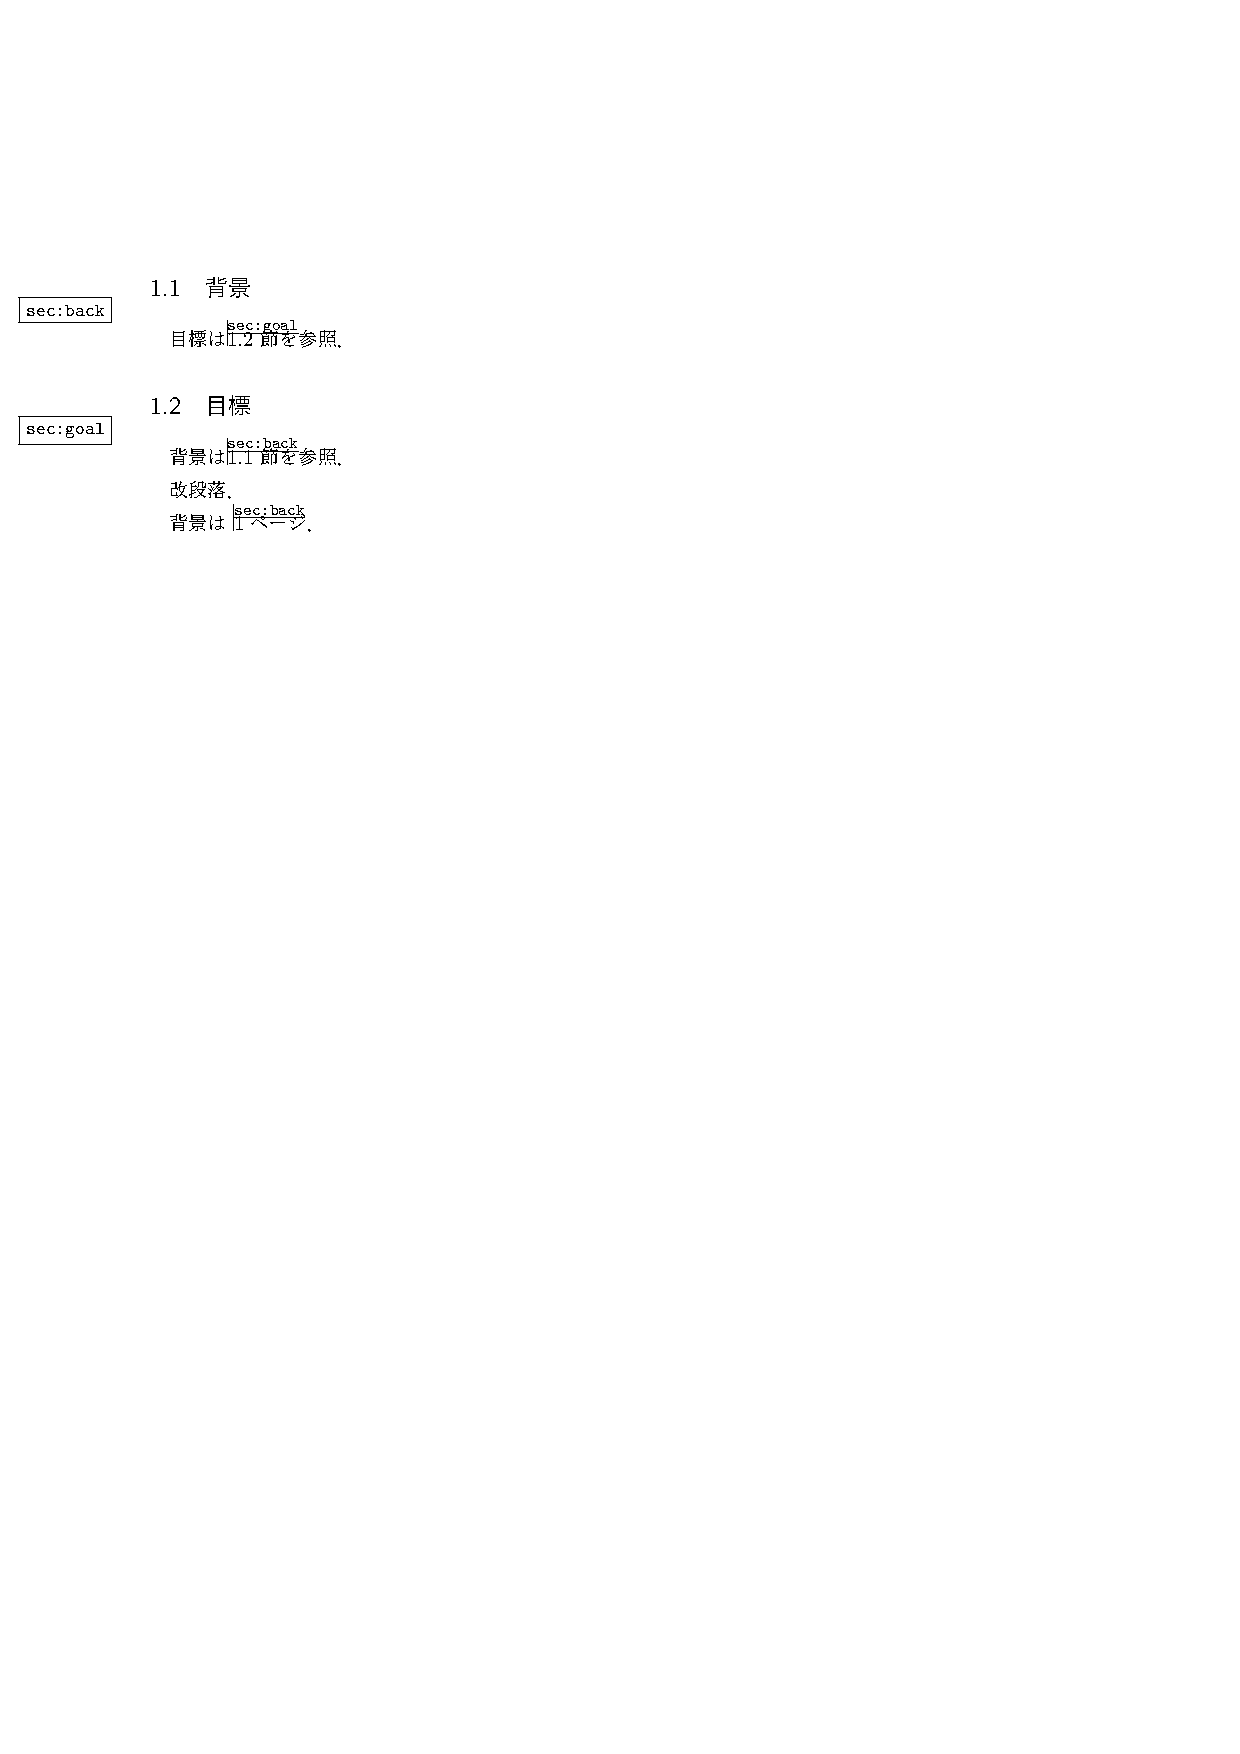
\includegraphics[clip,viewport=8 585 165 710]{images/showkeys}}}
\end{picture}
\begin{small}
\begin{verbatim}
\usepackage{showkeys}
\section{序論}
\subsection{背景}\label{sec:back}
目標は\ref{sec:goal}~節を参照.
\subsection{目標}\label{sec:goal}
背景は\ref{sec:back}~節を参照.\par
改段落.\par
背景は~\pageref{sec:back}ページ.
\end{verbatim}
\end{small}\IOlabel

\subsection{相互参照に関わる\LaTeX の警告}
%\zindind{相互参照}{に関わる警告}%
%コマンドプロンプトやシェルで表示される\dos{LaTeX Warning:}
%の後に以下に示すような警告が表示されていると,
%相互参照に関する問題が解消されていないことを示します.
%\par\dos{Label `key' multiply defined\hfil}
%というのは \cmd{label}命令で同じラベル名を持つラベルを定義している
%ということです.ラベルの重複がありますので,該当する
%ラベルに別の名前を付けます.
%
%\par\dos{Reference `key' on page n undefined\hfil}
%という警告が表示されたのならばラベル名が定義されていない
%ことになります.
%
%\par\noindent\dos{Label(s) may have 
%changed. Return to get cross-ferecenses right.\hfil} 
%が表示されたらラベルの値が変更されたということなので,
%もう1度タイプセットをします.この作業は1度で終わらない
%こともあるのでメッセージが表示されなくなるまでタイプセット
%を繰り返すこともあります.
%
%ラベルに関する問題はラベルの参照する名前などのスペルミスなど
%も考えられます.
\zindind{相互参照}{に関わる警告}%
コマンドプロンプトやシェルで表示される\dos{LaTeX Warning:}
の後に以下に示すような警告が表示されていると,
相互参照に関する問題が解消されていない事を示します.
\index{エラー!Label `key' multiply defined@\texttt{Label `key' multiply defined}}
\index{Label `key' multiply defined@\texttt{Label `key' multiply defined}}
\par\dos{Label `key' multiply defined\hfil}
というのは \cmd{label}命令で同じラベル名を持つラベルを定義している
という事です.ラベルの重複がありますので,該当する
ラベルに別の名前を付けます.

\index{エラー!Reference `key' on page n undefined@\texttt{Reference `key' on page n undefined}}
\index{Reference `key' on page n undefined@\texttt{Reference `key' on page n undefined}}
\par\dos{Reference `key' on page n undefined\hfil}
という警告が表示されたのならばラベル名が定義されていない
事になります.

\index{エラー!Label(s) may have 
changed. Return to get cross-ferecenses right.@\texttt{Label(s) may have changed. Return to get cross-ferecenses right.}}
\index{Label(s) may have changed. Return to get cross-ferecenses right.@\texttt{Label(s) may have changed. Return to get cross-ferecenses right.}}
\par\dos{Label(s) may have 
changed. Return to get cross-ferecenses right.\hfil} 
が表示されたらラベルの値が変更されたという事なので,
もう1度タイプセットをします.この作業は1度で終わらない
事もあるのでメッセージが表示されなくなるまでタイプセット
を繰り返す事もあります.

ラベルに関する問題はラベルの参照する名前などのスペルミスなど
も考えられます.


%\begin{metacomment}
% 以下のマークアップによる利点を説明するようなレベルにまで初級編は発展できないと思うので,コメントとする.
%\end{metacomment}

\begin{comment}

\section{マークアップによる利点}

さて,これまで\laTEX におけるコマンドの構成方法と機能・原理について
見てきた訳ですが,このような手段が提供されていると何が利点となるのでしょうか.

それは\LaTeX においてマークアップによる記述をする事により,\K{任意の要素に
意味付けを行う事ができる}という事です.

\chapref{kousei}では文書の体裁と調整するコマンド,例えば書体の大きさを
変更する \C{Large},要素を中央揃えにする \Env{center} 環境はどれも
\K{視覚的に体裁を直接変更する}というコマンドに他なりません.
そのため,これらを直接原稿中で記述しても何ら意味付けまではしていない事
になります.

%\begin{Exe}
%仮にその場しのぎ的に
%\end{Exe}

\begin{Prob}
これがどのような問題を引き起こすのか,非常に大規模な文書を執筆している時
に,それが理解できるでしょう.

始めからマクロ化・または一般化する事によってどのような利点があるのか,
自分なりに考察してください.
\end{Prob}


%\subsection{意味の記述}

もしも任意の要素の意味とレイアウトを同時に記述しようと思えば,
WYSIWYG 方式によるワードプロセッサでは相当困難な手順を踏む事に
なるでしょうし,要素の意味を確認しながらの作業は難しいでしょう.
何せ,ほとんどの WYSIWYG 方式のワードプロセッサは視覚レイアウト
を優先し,その文章に書かれている要素の意味までは把握しないのが
普通だからです.

% 何が問題なのか.
%\LaTeX のような処理系ではこのような問題も解決でき,要素の
%意味を確認しながら原稿を執筆する事が可能です.

%\subsection{一貫性}

%\begin{Exe}
%大規模な文書を作成しようと思えば\K{原稿を執筆する前に一貫性に関する
%ルールを決定する}必要があるという事です\footnote{もちろん,締め切り前日
%にその場しのぎ的にゼミのレジュメを完成させなければならないという状況
%においてはこの限りではありません.}.
%\end{Exe}


%\subsection{用語の統一}
%
%\subsection{一意性}
%
%ラベル参照の場合でも同じ
\end{comment}

